\section{Fun with Towers of Hanoi}
The Towers of Hanoi is a puzzle that consists of three pegs (\(A\), \(B\), and \(C\)) and a number of disks of different sizes, which can slide onto any peg. The puzzle starts with the disks arranged in a stack in ascending order of size on one peg, with the smallest disk at the top, forming a conical shape.

\begin{figure}[H]
    \centering
    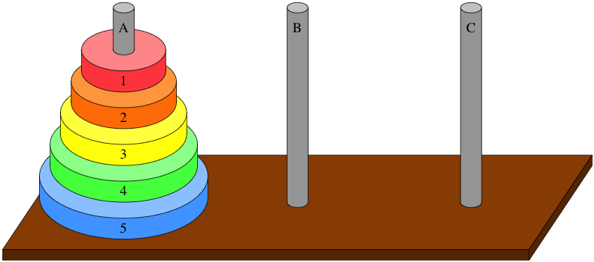
\includegraphics[width=0.4\linewidth]{images/5b5fb2670c9a185b2666637461e40c805fcc9ea5.png}
\end{figure}

The objective of the puzzle is to move all disks from peg \(A\) to peg \(B\) using the auxiliary peg $C$, while obeying the following rules:
\begin{enumerate}
    \item Only one disk may be moved at a time.
    \item Each move consists of taking the upper disk from one of the stacks and placing it on top of another stack or on an empty peg.
    \item No larger disk may be placed on top of a smaller disk.
\end{enumerate}

Here is an illustration of the steps needed to solve the puzzle for three disks:

\begin{figure}[H]
    \centering
    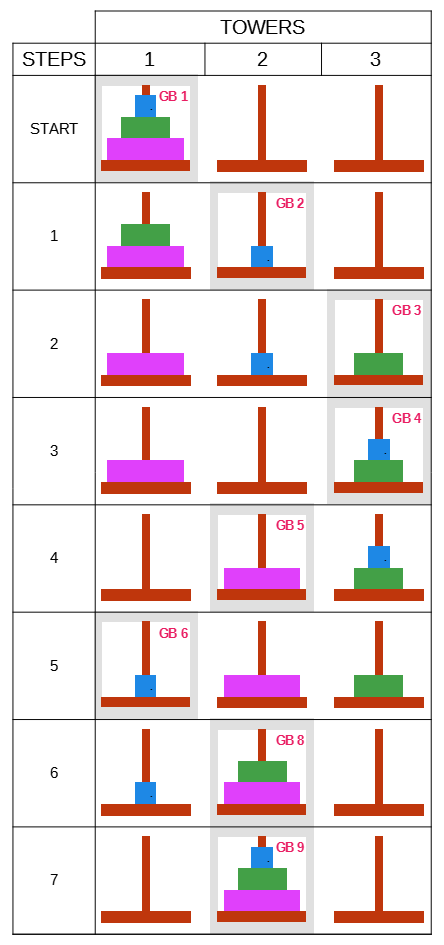
\includegraphics[width=0.3\linewidth]{images/000LCV-2.png}
\end{figure}


We want to write a predicate \texttt{move(N, Source, Target, Aux)} that prints the exact sequence of individual moves required to solve the puzzle for $N$ disks.

\titledbox{Think Recursively}{
If we think about the problem recursively, when we have $N>1$ disks, we want to move the top $N-1$ disks to the auxiliary peg, then move the one biggest disk to the target peg, then move the $N-1$ disks from the auxiliary to the target peg. The base case is trivial: moving one disk requires just a single direct move from source to target!
}

\titledbox{Prolog Printing}{
\begin{itemize}
    \item We will use the \texttt{write(X)} predicate that prints the value of \(X\) (\(X\) can be simple text or any type of argument) to the screen.
    \item We will use \inlinecode{nl} that prints a new line.
\end{itemize}
}

Let's write the base case (one disk):

\begin{codeblock}
move(1, A, B, _) :- !,
    write("Move top disk from "),
    write(A), write(" to "), write(B), nl.
\end{codeblock}

This is what we will get when we call it:

\begin{codeblock}
?- move(1, left,center,right).
Move top disk from left to center
true
\end{codeblock}

The recursion:

\begin{codeblock}
move(N,A,B,C) :-
    N>1,
    N1 is N-1,
    move(N1,A,C,B),
    move(1,A,B,_),
    move(N1,C,B,A).
\end{codeblock}

Let's test this:
\begin{codeblock}
?- move(3, left, center,right).
Move top disk from left to center
Move top disk from left to right
Move top disk from center to right
Move top disk from left to center
Move top disk from right to left
Move top disk from right to center
Move top disk from left to center
true
\end{codeblock}


\newpage
\begin{excursion}[Towers of Hanoi Time Complexity]{}
Let $T(N)$ be the number of moves needed to move $N$ disks. 

If there is only one disk, you move it once (base case):
\[
T(1) = 1
\]

For the recursive case, we want to move $N>1$ disks from peg $A$ to $B$ using $C$:
\begin{enumerate}
    \item Move $N-1$ disks from $A$ to $C$ (\textit{that takes $T(N-1)$ moves})
    \item Move the largest disk from $A$ to $B$ (\textit{one move})
    \item Move the $N-1$ disks from $C$ to $B$ (\textit{another $T(N-1)$ moves})
\end{enumerate}

Therefore:

\[
T(N) = T(N-1) + 1 + T(N-1) = 2T(N-1)+1
\]


Computing $T(N-1)$ the same way gives us 

\[
T(N-1) = T(N-2) + 1 + T(N-2) = 2T(N-2)+1
\]

Substitute:
\[
2T(N-1)+1 = 2(2T(N-2)+1)+1
\]


Expand:

\[
2(2T(N-2)+1)+1 = (4T(N-2) + 2) + 1 = 4T(N-2) + 3
\]

Computing $T(N-2)$ the same way gives us 
\[
T(N-2) = T(N-3) + 1 + T(N-3) = 2T(N-3)+1
\]


Substitute:
\[
4T(N-2) + 3 = 4(2T(N-3)+1) + 3
\]

Expand:
\[
(8T(N-3) + 4) + 3 = 8T(N-3) + 7
\]

And so on $\cdots$


\observationbox{
For a recursive step $k$, we get the following:
\begin{itemize}
    \item $k=1 \to T(N) = 2T(N-1)+1$
    \item $k=2 \to  T(N) = 4T(N-2) + 3$
    \item $k=3 \to T(N) = 8T(N-3) + 7$
\end{itemize}
}


This can be generalized to:

\[
T(N) = 2^k T(N-k) + (2^k - 1)
\]


We stop the recursion when we reach the base case $T(1)$ which occurs when $N-k = 1$ (that is, when $k=N-1$).


For $k = N-1$, we have

\begin{align*}
T(N) &= 2^{N-1} T(N - (N - 1)) + (2^{N-1} - 1) \\
     &= 2^{N-1} T(1) + (2^{N-1} - 1) \\
     &= 2^{N-1} + (2^{N-1} - 1) \\
     &= 2 \cdot 2^{N-1} - 1 \\
     &= 2^N - 1
\end{align*}
\redbox{The complexity is $\mathcal{O}(2^N - 1) = \mathcal{O}(2^N)$, i.e., \textbf{exponential}. For our 3-disk example, $T(3) = 2^3 - 1 = 7$ moves, exactly matching the 7 lines of output above.}
\end{excursion}